\documentclass[11pt]{article}
\usepackage[a4paper, left=1.5cm,right=1.5cm,top=2cm,bottom=2cm]{geometry}

%%%%%%%%%%%%%%%%%%%%%%%%%%%%%%%%%%%%%%%%%%%%%%%%%%%%%%%%%%%%%%%%%%%%%%%%%%%%%%%%
% Page layout and formatting
\usepackage{authblk}        % For author affiliations
\setlength{\parindent}{0pt} % No indentation for paragraphs
\usepackage{setspace}       % For line spacing
\setstretch{1.2}            % Set line spacing to 1.2
%%%%%%%%%%%%%%%%%%%%%%%%%%%%%%%%%%%%%%%%%%%%%%%%%%%%%%%%%%%%%%%%%%%%%%%%%%%%%%%%
% Mathematical packages
\usepackage{amsmath}   % For mathematical symbols and equations
\usepackage{amssymb}   % For additional mathematical symbols
\usepackage{bm}        % For bold math symbols
%%%%%%%%%%%%%%%%%%%%%%%%%%%%%%%%%%%%%%%%%%%%%%%%%%%%%%%%%%%%%%%%%%%%%%%%%%%%%%%%
% Graphics and diagrams
\usepackage{tikz}   % For drawing diagrams
%%%%%%%%%%%%%%%%%%%%%%%%%%%%%%%%%%%%%%%%%%%%%%%%%%%%%%%%%%%%%%%%%%%%%%%%%%%%%%%%
% Tables
\usepackage{booktabs} % for \toprule \midrule \bottomrule
%%%%%%%%%%%%%%%%%%%%%%%%%%%%%%%%%%%%%%%%%%%%%%%%%%%%%%%%%%%%%%%%%%%%%%%%%%%%%%%%
% Fonts
\usepackage[T1]{fontenc}
\usepackage{mlmodern}
%%%%%%%%%%%%%%%%%%%%%%%%%%%%%%%%%%%%%%%%%%%%%%%%%%%%%%%%%%%%%%%%%%%%%%%%%%%%%%%%
% Bibliography
\usepackage[numbers]{natbib}
%%%%%%%%%%%%%%%%%%%%%%%%%%%%%%%%%%%%%%%%%%%%%%%%%%%%%%%%%%%%%%%%%%%%%%%%%%%%%%%%
%hyperlinks
\usepackage{hyperref}
\hypersetup{colorlinks,
  linkcolor=blue,
  citecolor=blue,
  urlcolor=blue}
%%%%%%%%%%%%%%%%%%%%%%%%%%%%%%%%%%%%%%%%%%%%%%%%%%%%%%%%%%%%%%%%%%%%%%%%%%%%%%%%
% Title
\title{\large \textbf{A Compositional Autoencoder for Steady Flow past Objects
in a Lid-Driven Cavity: Experiments and Diagnostics}}

%%%%%%%%%%%%%%%%%%%%%%%%%%%%%%%%%%%%%%%%%%%%%%%%%%%%%%%%%%%%%%%%%%%%%%%%%%%%%%%%
% Author and affiliation
\author[]{Suresh Murugaiyan}
\affil[]{Translational AI Center, Iowa State University, Ames, IA}
%%%%%%%%%%%%%%%%%%%%%%%%%%%%%%%%%%%%%%%%%%%%%%%%%%%%%%%%%%%%%%%%%%%%%%%%%%%%%%%%
\author[]{Hayden Garcia Chelstrom}
\affil[]{Translational AI Center, Iowa State University, Ames, IA}
%%%%%%%%%%%%%%%%%%%%%%%%%%%%%%%%%%%%%%%%%%%%%%%%%%%%%%%%%%%%%%%%%%%%%%%%%%%%%%%%
\author[]{Vienna Rossmanith}
\affil[]{Translational AI Center, Iowa State University, Ames, IA}
%%%%%%%%%%%%%%%%%%%%%%%%%%%%%%%%%%%%%%%%%%%%%%%%%%%%%%%%%%%%%%%%%%%%%%%%%%%%%%%%
\author[]{Baskar Ganapathysubramanian}
\affil[]{Translational AI Center, Iowa State University, Ames, IA}
%%%%%%%%%%%%%%%%%%%%%%%%%%%%%%%%%%%%%%%%%%%%%%%%%%%%%%%%%%%%%%%%%%%%%%%%%%%%%%%%
\date{July 8, 2026}
%%%%%%%%%%%%%%%%%%%%%%%%%%%%%%%%%%%%%%%%%%%%%%%%%%%%%%%%%%%%%%%%%%%%%%%%%%%%%%%%
% chktex-file 17
% chktex-file 9
% chktex-file 8

\date{July 2026}

\begin{document}

\maketitle

\section{Introduction}

This project asks a simple question: when a neural network compresses a
flow field into a short list of numbers, can we make those numbers
\emph{mean} something physical?

The tool we use is an \emph{autoencoder}: a pair of networks in which an
\emph{encoder} squeezes a full flow field (hundreds of thousands of grid
values) down to a short vector $\boldsymbol{z}$, and a \emph{decoder}
rebuilds the field from that vector alone. The short vector is called the
\emph{latent vector}, and the space it lives in is the \emph{latent
space}. Readers who know proper orthogonal decomposition (POD) can think
of an autoencoder as a nonlinear POD: instead of modal amplitudes, the
network learns its own compressed coordinates. We train on the FlowBench
2D lid-driven cavity dataset: steady Navier--Stokes flow in a square
cavity whose top lid moves at constant speed, with a solid object placed
inside the cavity.

Ordinarily the latent vector is a black box: the network stores
information wherever it likes, and no single entry means anything. Our
key structural choice is to split $\boldsymbol{z}$, by architecture, into
three named blocks, each intended to carry exactly one physical factor:
%
\begin{equation}
  \boldsymbol{z} \;=\;
  [\, \underbrace{\boldsymbol{z}_{\mu}}_{\text{regime }(4)}
  \,\|\,
  \underbrace{\boldsymbol{z}_{g}}_{\text{geometry }(32)}
  \,\|\,
  \underbrace{\boldsymbol{z}_{\xi}}_{\text{residual }(16)} \,]
  \;\in\; \mathbb{R}^{52}.
\end{equation}
%
In words: 52 numbers summarize each flow field. The first 4
($\boldsymbol{z}_{\mu}$, the \emph{regime} block) should describe the
operating condition --- here, the Reynolds number Re. The next 32
($\boldsymbol{z}_{g}$, the \emph{geometry} block) should describe the
shape of the object in the cavity. The last 16 ($\boldsymbol{z}_{\xi}$,
the \emph{residual} block) are free capacity for whatever else the
reconstruction needs.

The hypothesis under test: after training, $\boldsymbol{z}_{\mu}$ should
contain the Reynolds number, $\boldsymbol{z}_{g}$ should contain the
object shape, and neither should \emph{leak} into the other --- that is,
you should not be able to recover Re by reading the geometry block.
Because the flow here is steady (it does not change in time), there is no
dynamics block $\boldsymbol{z}_{\eta}$ and no latent time-stepper $\Phi$
in this first version; those enter later with time-dependent cases.

\section{Dataset}

This section describes what one training sample looks like and which
labels we extract from it. Each FlowBench sample is a steady lid-driven
cavity solution stored on a $512 \times 512$ grid. The data loader
(\texttt{data/dataset.py}) unpacks the raw \texttt{.npz} arrays into:
%
\begin{itemize}
  \item \textbf{fields} --- the solution itself: horizontal velocity $u$,
        vertical velocity $v$, and pressure $p$ at every grid point.
        We resize $512^2 \to 256^2$ to make training cheaper; this loses
        little information for these smooth steady fields.
  \item \textbf{sdf} --- the signed distance field of the object: at
        every grid point, the distance to the object's surface, with a
        positive sign in the fluid and a negative sign inside the solid.
        The SDF is a convenient, smooth description of the shape, and it
        serves as our geometry label.
  \item \textbf{mask} --- a binary image: $1$ where there is fluid, $0$
        inside the solid object.
  \item \textbf{log\_re} --- the regime label. Re is stored in the file
        as a constant image, so we read a single pixel to get the number.
        We use $\log_{10}\mathrm{Re}$ rather than Re because Re spans
        orders of magnitude, and we \emph{standardize} it (subtract the
        mean, divide by the standard deviation) so the network sees
        values of order one. The mean and standard deviation are computed
        on the \emph{training} set only, and the test set reuses them, so
        both splits are measured on exactly the same scale.
\end{itemize}
%
The loader also computes three simple geometry summaries from the mask:
the fraction of the cavity occupied by the solid (area fraction) and the
$x$ and $y$ coordinates of the solid's center (centroid). These three
numbers are never used during training. They exist only as ground-truth
targets for the diagnostic of Section~\ref{sec:diagnostics}: if the
geometry block truly contains the shape, simple shape summaries should be
readable from it.

\section{Network architecture}

Four modules make up the model
(\texttt{models/compositional/networks.py}):
%
\begin{itemize}
  \item \textbf{FieldEncoder} $\mathcal{E}$ --- a convolutional neural
        network (CNN): a stack of learned filters that repeatedly halves
        the image resolution ($256 \to 128 \to \dots \to 8$), so that
        each stage sees increasingly large-scale features of the flow.
        After the final stage the features are pooled and passed through
        \emph{three separate linear layers} (``heads''), one producing
        $\boldsymbol{z}_{\mu}$, one $\boldsymbol{z}_{g}$, and one
        $\boldsymbol{z}_{\xi}$. The blocks are therefore separate objects
        from the very start.
  \item \textbf{FieldDecoder} $\mathcal{D}$ --- the mirror image of the
        encoder: the full vector $\boldsymbol{z}$ is reshaped into a
        small $8 \times 8$ feature map and repeatedly upsampled back to a
        $256^2$ $(u, v, p)$ field.
  \item \textbf{RegimeHead} --- a small network that is shown
        $\boldsymbol{z}_{\mu}$ \emph{only} and must predict
        $\log \mathrm{Re}$.
  \item \textbf{SDFHead} --- a small decoder that is shown
        $\boldsymbol{z}_{g}$ \emph{only} and must redraw the object's SDF
        at $64 \times 64$ resolution.
\end{itemize}
%
The two small heads are the supervision mechanism, and the logic is worth
spelling out. The regime head can only see $\boldsymbol{z}_{\mu}$; if it
is required to predict Re, then the encoder has no choice but to route
Reynolds-number information into that block. Likewise, the SDF head can
only see $\boldsymbol{z}_{g}$, so shape information must flow there.
Note what this does \emph{not} guarantee: it forces the right information
\emph{into} the right block, but nothing yet prevents extra copies of the
same information from also appearing in the wrong blocks. That gap drives
most of the experiments below.

\section{Training objective}

A \emph{loss} is a number that measures how wrong the network currently
is; training is the process of adjusting the network's parameters to make
a weighted sum of losses as small as possible. Each optimization step
combines four losses (\texttt{models/compositional/compositional\_ae.py}),
weighted by $\lambda$-coefficients set in the configuration file:
%
\begin{enumerate}
  \item \textbf{Masked reconstruction (L1).} The mean squared error (MSE)
        between the decoded field and the true field, evaluated over
        fluid points only. Predictions inside the solid are zeroed out,
        and the error is divided by the number of fluid points, so a
        sample with a large object is not unfairly weighted. This loss
        makes the autoencoder reconstruct accurately.
  \item \textbf{Regime supervision.} MSE between the regime head's
        prediction and the true standardized $\log_{10}\mathrm{Re}$.
        This pulls Re into $\boldsymbol{z}_{\mu}$.
  \item \textbf{Geometry supervision.} MSE between the SDF head's output
        and the true (downsampled) SDF. This pulls the shape into
        $\boldsymbol{z}_{g}$.
  \item \textbf{Cross-block decorrelation (L6).} The Pearson correlation
        between two quantities measures their linear relationship: $+1$
        or $-1$ means perfectly related, $0$ means no linear relation.
        Across each training batch we compute the correlation between
        every entry of one block and every entry of another block, and
        penalize its average absolute value, for all three block pairs.
        The idea: losses~2--3 pull information \emph{into} the correct
        block; this term is meant to push redundant copies \emph{out of}
        the wrong blocks by discouraging any linear relationship between
        blocks.
\end{enumerate}
%
The residual block $\boldsymbol{z}_{\xi}$ receives no supervision at all.
It is free capacity that absorbs whatever the reconstruction needs beyond
(Re, shape) --- exactly the role the framework assigns to the residual
block.

Training is driven by \texttt{main.py}: it loads the YAML configuration,
fixes the random seeds (so results are repeatable), builds the train and
test datasets (passing the training Re statistics to the test set), and
trains with PyTorch Lightning, keeping the checkpoint with the best
validation reconstruction error.

\section{Linear-probe diagnostics}
\label{sec:diagnostics}

Training tells us the losses went down; it does not tell us whether the
blocks actually mean what we intended. The diagnostic
(\texttt{diagnostics/probes.py}) is the actual scientific test, and it
works as follows. After training, we encode the entire test set. Then,
for each block and each known physical quantity, we fit a \emph{linear
probe}: a plain linear regression that tries to predict the quantity
(say, $\log \mathrm{Re}$) from the entries of one block (say,
$\boldsymbol{z}_{g}$) alone. We use \emph{ridge} regression (linear
regression with a small penalty on the coefficients, which keeps the fit
stable) and 5-fold cross-validation (fit on four fifths of the data, test
on the remaining fifth, rotate five times, average), so the score
reflects genuine predictive power rather than memorization.

The score is $R^2$, the fraction of the target's variance the probe
explains: $R^2 = 1$ means the quantity is perfectly readable from the
block with a linear formula; $R^2 \approx 0$ means the block carries no
usable linear information about it; negative values mean the probe does
worse than simply guessing the average. For a compositional latent we
expect the block-diagonal pattern of Table~\ref{tab:probes}: each
quantity readable from its own block and from nowhere else.

\begin{table}[htbp]
  \centering
  \caption{Expected linear-probe $R^2$ pattern for a compositional latent
  space. High $R^2$ on the matching block and low $R^2$ elsewhere indicates
  a successful factorization; a high off-diagonal entry indicates leakage.}
  \label{tab:probes}
  \begin{tabular}{lccc}
    \toprule
    Target & $\boldsymbol{z}_{\mu}$ & $\boldsymbol{z}_{g}$ & $\boldsymbol{z}_{\xi}$ \\
    \midrule
    $\log \mathrm{Re}$    & \textbf{high} & low           & low \\
    Area fraction         & low           & \textbf{high} & low \\
    Centroid $x$          & low           & \textbf{high} & low \\
    Centroid $y$          & low           & \textbf{high} & low \\
    \bottomrule
  \end{tabular}
\end{table}

If the trained latent reproduces this pattern, the factorization worked:
Re is linearly readable from the regime block and \emph{not} from the
geometry block, and vice versa. A high $R^2$ in an off-diagonal cell
means information \emph{leaked} into a block where it does not belong ---
exactly what the loss-ablation experiments below are designed to study.

\section{Results}

\subsection{Overview}

Seven training runs to date, each changing one ingredient at a time so
that any change in the outcome can be attributed to that ingredient.
Table~\ref{tab:overview} summarizes the arc. In brief: the baseline
(Run 1) puts the right information in the right blocks but also leaks Re
everywhere; making the statistical decorrelation penalty stronger (Runs
2--3) trades quality for leakage without fixing the problem; the two
\emph{structural} losses --- same-factor invariance (L10, Run 4) and swap
consistency (L12, Run 5) --- deliver clean separation and clean
recombination at matched conditions; the cross-Re swap loss (Run 6)
delivers \emph{transfer}: the ability to predict a geometry at a new
Reynolds number, which every earlier model failed by two orders of
magnitude; and the static geometry encoder (Run 7) closes the remaining
leak by computing $\boldsymbol{z}_{g}$ directly from the SDF, confirming
the mechanism found by the concept-vector diagnostic. Run 7 is the
current best configuration. The following subsections document each run
in chronological order, each ending with the reasoning that led to the
next run.

\begin{table}[htbp]
  \centering
  \caption{Summary of all runs. ``Leakage'' is the linear-probe $R^2$ of
  $\log \mathrm{Re}$ read from $\boldsymbol{z}_{g}$, where it does not
  belong (target $\lesssim 0.3$); the swap ratios compare swap error to
  reconstruction error (target $\approx 1$; defined in
  Section~\ref{sec:swap}).}
  \label{tab:overview}
  \begin{tabular}{llcccl}
    \toprule
    Run & Configuration & Leakage & Same-Re & Cross-Re & Verdict \\
    \midrule
    1 & $\lambda_{\mathrm{decorr}} = 0.01$ & 0.900 & 1.06 & 260 & Re leaks into all blocks \\
    2 & $\lambda_{\mathrm{decorr}} = 0.5$  & 0.719 & ---  & --- & trade-off: quality lost, leak remains \\
    3 & $\lambda_{\mathrm{decorr}} = 0.1$  & 0.865 & ---  & --- & statistical penalty insufficient \\
    4 & $+$ invariance L10                 & \textbf{0.215} & 1.35 & 194 & separated, but brittle \\
    5 & $+$ swap L12                       & 0.343 & \textbf{1.04} & 199 & recombinable, no transfer \\
    6 & $+$ cross-Re swap                  & 0.405 & 1.57 & 2.1 & \emph{transfer learned} \\
    7 & $+$ static geometry encoder        & $\mathbf{-0.15}$ & 1.42 & \textbf{1.4} & mechanism confirmed; best overall \\
    \bottomrule
  \end{tabular}
\end{table}

\begin{figure}[htbp]
  \centering
  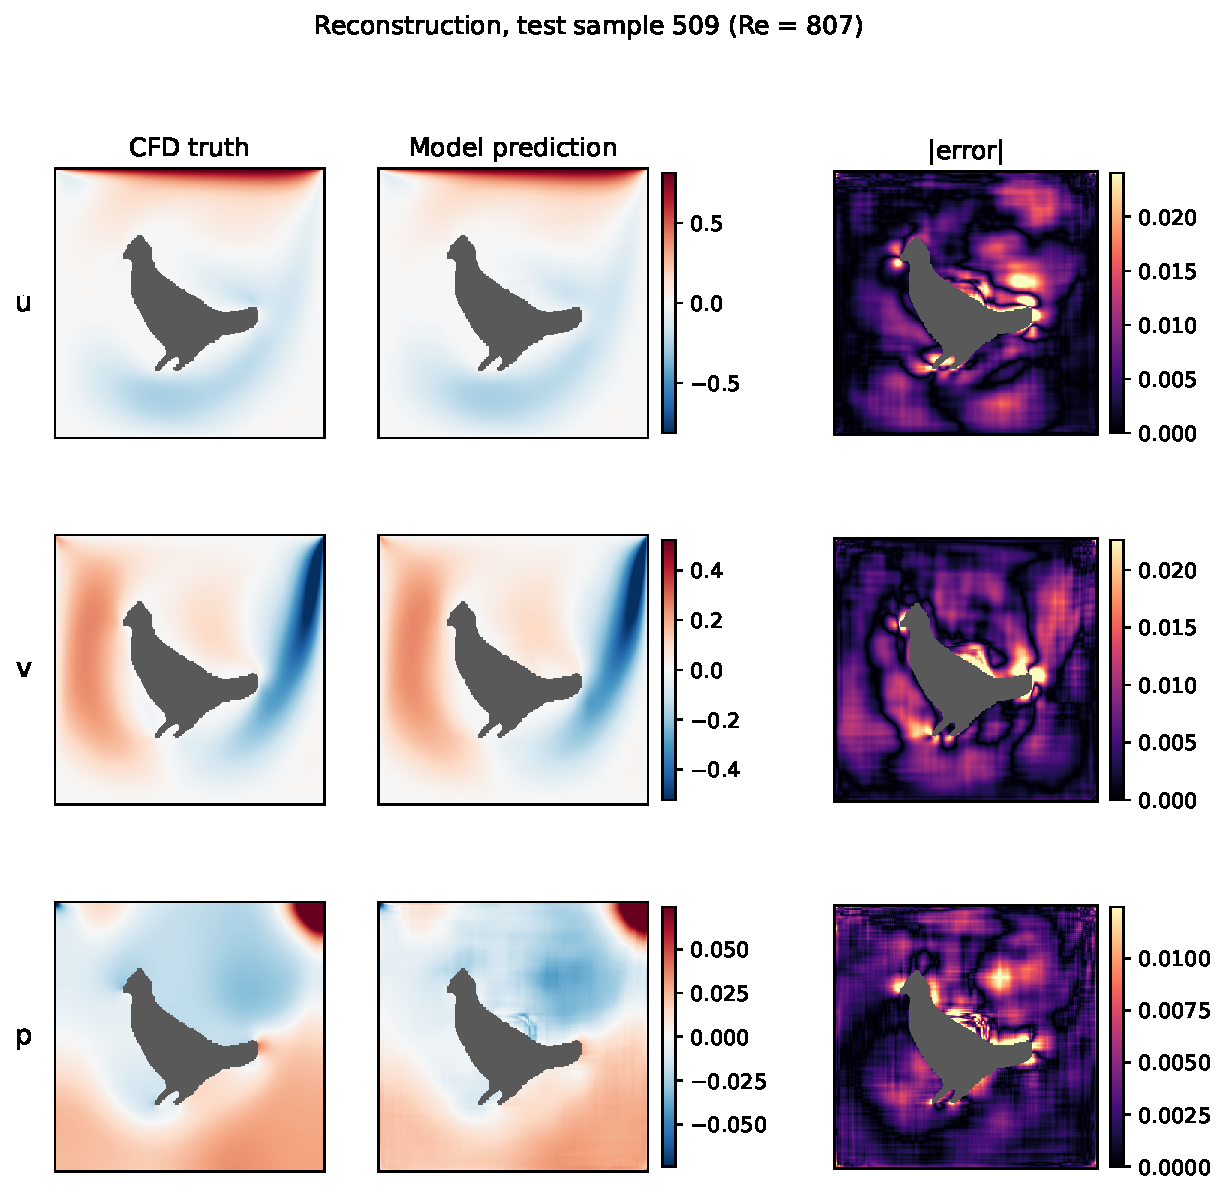
\includegraphics[width=0.92\textwidth]{figures/reconstruction_509.pdf}
  \caption{What reconstruction looks like: a test sample from the final
  model (Run 7). Rows are the three field channels $(u, v, p)$; columns
  are the CFD truth, the model's reconstruction from the 52-number
  latent, and the absolute error (note the error color scale is roughly
  ten times finer than the field scale). The solid object is shown in
  gray. Errors concentrate in thin layers at the object surface.}
  \label{fig:recon}
\end{figure}

\subsection{Run 1: baseline loss weights}

First training run on the FlowBench LDC ``easy'' split (2{,}400 training
/ 600 test samples): 200 epochs (an epoch is one full pass through the
training data), batch size 16, resolution $256^2$, loss weights
$\lambda_{\mathrm{recon}} = 1.0$, $\lambda_{\mathrm{regime}} =
\lambda_{\mathrm{geo}} = 0.1$, $\lambda_{\mathrm{decorr}} = 0.01$
(single NVIDIA GPU, $\sim$18 minutes). The final masked reconstruction
error was $2.7 \times 10^{-3}$ on the training set and $2.1 \times
10^{-3}$ on the validation set --- similar values, so the network is not
merely memorizing the training data. Table~\ref{tab:probes-run1} reports
the measured linear-probe $R^2$.

\begin{table}[htbp]
  \centering
  \caption{Run 1: measured linear-probe $R^2$ on the 600-sample test split
  ($\lambda_{\mathrm{decorr}} = 0.01$). Bold marks the block that should
  carry each target.}
  \label{tab:probes-run1}
  \begin{tabular}{lccc}
    \toprule
    Target & $\boldsymbol{z}_{\mu}$ & $\boldsymbol{z}_{g}$ & $\boldsymbol{z}_{\xi}$ \\
    \midrule
    $\log \mathrm{Re}$    & \textbf{0.994} & 0.900          & 0.777 \\
    Area fraction         & 0.042          & \textbf{0.688} & 0.172 \\
    Centroid $x$          & 0.027          & \textbf{0.736} & 0.373 \\
    Centroid $y$          & $-0.013$       & \textbf{0.690} & 0.214 \\
    \bottomrule
  \end{tabular}
\end{table}

\paragraph{What worked.} The regime block is clean:
$\boldsymbol{z}_{\mu}$ reads $\log \mathrm{Re}$ at $R^2 = 0.994$ and
contains essentially no geometry ($R^2 \le 0.04$). Geometry is readable
from $\boldsymbol{z}_{g}$ ($R^2 \approx 0.69$--$0.74$) and nearly absent
from $\boldsymbol{z}_{\mu}$. The moderate (rather than near-perfect)
geometry scores are not alarming: the probes are \emph{linear}, while
area and centroid depend on the encoded shape in a nonlinear way, so even
a perfect geometry block would not give $R^2 = 1$ here.

\paragraph{What failed.} Reynolds-number information leaked into the
other blocks: $\log \mathrm{Re}$ is readable from $\boldsymbol{z}_{g}$
at $R^2 = 0.900$ and from $\boldsymbol{z}_{\xi}$ at $0.777$. The reason
is easy to see. The decoder needs Re to rebuild the field, and nothing
stops the encoder from stashing a copy of Re in \emph{every} block --- in
fact the reconstruction loss rewards extra copies, because they can only
help the decoder. A well-known theoretical result (Locatello et al.)
says precisely this: without extra constraints, a network that
reconstructs well is free to scramble the underlying factors across its
latent however it likes. The decorrelation penalty is supposed to prevent
the copies, but at $\lambda_{\mathrm{decorr}} = 0.01$ it is roughly a
hundred times weaker than the reconstruction term, and it loses the
competition.

\paragraph{Next experiment.} The leaked Re is \emph{linearly} readable
from $\boldsymbol{z}_{g}$ --- and a linear relationship is exactly what a
Pearson penalty acts on. So the next run raises
$\lambda_{\mathrm{decorr}}$ from $0.01$ to $0.5$, changing nothing else.
Success would mean: the off-diagonal $\log \mathrm{Re}$ entries drop
substantially (toward $R^2 \lesssim 0.3$) while reconstruction and the
geometry row stay near their Run-1 values. If even a strong Pearson
weight cannot remove the leakage, the natural escalation is HSIC (L7, a
penalty that detects nonlinear dependence too) and the swap-consistency
loss (L12), which attacks the problem functionally rather than
statistically.

\subsection{Run 2: strong Pearson decorrelation}

Identical to Run~1 except $\lambda_{\mathrm{decorr}} = 0.5$, a $50\times$
increase. Table~\ref{tab:probes-run2} reports the measured linear-probe
$R^2$, with the Run-1 values in parentheses for comparison.

\begin{table}[htbp]
  \centering
  \caption{Run 2: measured linear-probe $R^2$ on the test split
  ($\lambda_{\mathrm{decorr}} = 0.5$), with Run-1 values
  ($\lambda_{\mathrm{decorr}} = 0.01$) in parentheses. Bold marks the
  block that should carry each target.}
  \label{tab:probes-run2}
  \begin{tabular}{lccc}
    \toprule
    Target & $\boldsymbol{z}_{\mu}$ & $\boldsymbol{z}_{g}$ & $\boldsymbol{z}_{\xi}$ \\
    \midrule
    $\log \mathrm{Re}$ & \textbf{0.886} (0.994) & 0.719 (0.900) & 0.487 (0.777) \\
    Area fraction      & $-0.002$ (0.042)       & \textbf{0.402} (0.688) & 0.262 (0.172) \\
    Centroid $x$       & $-0.016$ (0.027)       & \textbf{0.565} (0.736) & 0.378 (0.373) \\
    Centroid $y$       & 0.016 ($-0.013$)       & \textbf{0.427} (0.690) & 0.115 (0.214) \\
    \bottomrule
  \end{tabular}
\end{table}

\paragraph{Outcome: a trade-off, not a fix.} The leakage did shrink ---
$\log \mathrm{Re}$ from $\boldsymbol{z}_{g}$ dropped from $0.900$ to
$0.719$, and from $\boldsymbol{z}_{\xi}$ from $0.777$ to $0.487$ --- but
everything else got worse too: the on-diagonal regime readout degraded
($0.994 \to 0.886$) and geometry recovery from $\boldsymbol{z}_{g}$ fell
by roughly $0.2$ on all three descriptors. This is what economists call a
\emph{Pareto trade-off}: one goal improves only by sacrificing another,
with no setting that improves both. The underlying reason is that the
Pearson penalty is a blunt instrument. It cannot tell the difference
between a redundant \emph{copy} of information (which we want removed)
and informative, structured coordinates (which we want kept); at a large
weight it simply flattens all correlations, scrambling every block a
little --- while the leakage still sits far above the $R^2 \lesssim 0.3$
target. A $50\times$ stronger penalty bought a modest leakage reduction
at a real cost: strong evidence that tuning the weight of a statistical
independence penalty will not, by itself, separate the blocks.

\paragraph{Next experiments.} Two directions, in order:
(i)~$\lambda_{\mathrm{decorr}} = 0.1$ as an intermediate point --- with
Runs 1--2 it maps out how the trade-off curve behaves between the two
extremes; (ii)~\emph{same-factor invariance} (L10). The dataset contains
each geometry simulated at several Reynolds numbers, and that structure
can be exploited directly: penalize any \emph{variation} of
$\boldsymbol{z}_{g}$ across samples that share a geometry. Since those
samples differ only in Re, this demands outright that
$\boldsymbol{z}_{g}$ not change when only Re changes --- a
\emph{functional} constraint on the encoder's behavior, rather than a
statistical property of a batch.

\subsection{Run 3: intermediate decorrelation --- the verdict on the sweep}

Identical to Runs~1--2 except $\lambda_{\mathrm{decorr}} = 0.1$.
Table~\ref{tab:probes-run3} assembles the complete three-point weight
sweep in one place.

\begin{table}[htbp]
  \centering
  \caption{Pearson-decorrelation weight sweep: linear-probe $R^2$ on the
  test split for $\lambda_{\mathrm{decorr}} \in \{0.01, 0.1, 0.5\}$
  (Runs 1, 3, 2). Bold marks the block that should carry each target.}
  \label{tab:probes-run3}
  \begin{tabular}{llccc}
    \toprule
    Target & $\lambda_{\mathrm{decorr}}$ & $\boldsymbol{z}_{\mu}$ & $\boldsymbol{z}_{g}$ & $\boldsymbol{z}_{\xi}$ \\
    \midrule
    $\log \mathrm{Re}$ & 0.01 & \textbf{0.994} & 0.900 & 0.777 \\
                       & 0.1  & \textbf{0.978} & 0.865 & 0.752 \\
                       & 0.5  & \textbf{0.886} & 0.719 & 0.487 \\
    \midrule
    Area fraction      & 0.01 & 0.042    & \textbf{0.688} & 0.172 \\
                       & 0.1  & 0.017    & \textbf{0.657} & 0.368 \\
                       & 0.5  & $-0.002$ & \textbf{0.402} & 0.262 \\
    \midrule
    Centroid $x$       & 0.01 & 0.027    & \textbf{0.736} & 0.373 \\
                       & 0.1  & 0.014    & \textbf{0.712} & 0.493 \\
                       & 0.5  & $-0.016$ & \textbf{0.565} & 0.378 \\
    \midrule
    Centroid $y$       & 0.01 & $-0.013$ & \textbf{0.690} & 0.214 \\
                       & 0.1  & 0.012    & \textbf{0.657} & 0.245 \\
                       & 0.5  & 0.016    & \textbf{0.427} & 0.115 \\
    \bottomrule
  \end{tabular}
\end{table}

\paragraph{Verdict on statistical decorrelation.} The intermediate weight
keeps nearly all of Run~1's quality (regime readout $0.978$, geometry
$0.66$--$0.71$) but buys almost no leakage reduction
($\log \mathrm{Re}$ from $\boldsymbol{z}_{g}$: $0.900 \to 0.865$). Across
the whole sweep, leakage falls only when representation quality is
heavily taxed: there is \emph{no} weight at which the Pearson penalty
removes the redundant Reynolds copy while preserving what the blocks are
supposed to contain. This is a clean negative result, and it matches the
framework's prediction: statistical independence penalties cannot make a
factorization \emph{functional}. The next run therefore switches to the
structural tool.

\paragraph{Setting up Run 4: same-factor invariance (L10).} Because each
geometry appears at several Reynolds numbers, we can build
\emph{group-structured minibatches}: instead of sampling training batches
at random, each batch is deliberately composed of a few geometry groups,
each contributing the same shape at several different Re. The new loss is
%
\begin{equation}
  \mathcal{L}_{\mathrm{inv}}
  \;=\;
  \mathbb{E}_{\text{groups}}
  \Bigl[ \bigl\| \boldsymbol{z}_{g}^{(i)} -
  \overline{\boldsymbol{z}_{g}}^{\,\text{group}} \bigr\|^2 \Bigr],
\end{equation}
%
the average squared distance between each sample's geometry code and the
mean geometry code of its group. Samples within a group differ
\emph{only} in Re; so if $\boldsymbol{z}_{g}$ contains any Re content at
all, it must vary within the group, and this loss punishes it directly.
Run 4 keeps $\lambda_{\mathrm{decorr}} = 0.01$ (the Run-1 value) and adds
only the invariance term, so any improvement is attributable to L10
alone.

\subsection{Run 4: same-factor invariance --- the structural loss succeeds}

Run 4 uses the Run-1 weights plus the same-factor invariance term with
$\lambda_{\mathrm{inv}} = 0.1$, trained on group-structured minibatches
(four geometry groups of four Reynolds numbers per batch of 16).
Table~\ref{tab:probes-run4} reports the probe $R^2$ against the Run-1
baseline.

\begin{table}[htbp]
  \centering
  \caption{Run 4: linear-probe $R^2$ with the same-factor invariance loss
  (L10), Run-1 values in parentheses. Bold marks the block that should
  carry each target.}
  \label{tab:probes-run4}
  \begin{tabular}{lccc}
    \toprule
    Target & $\boldsymbol{z}_{\mu}$ & $\boldsymbol{z}_{g}$ & $\boldsymbol{z}_{\xi}$ \\
    \midrule
    $\log \mathrm{Re}$ & \textbf{0.986} (0.994) & 0.215 (0.900) & 0.412 (0.777) \\
    Area fraction      & $-0.003$ (0.042)       & \textbf{0.677} (0.688) & 0.130 (0.172) \\
    Centroid $x$       & 0.009 (0.027)          & \textbf{0.756} (0.736) & 0.143 (0.373) \\
    Centroid $y$       & 0.011 ($-0.013$)       & \textbf{0.711} (0.690) & 0.047 (0.214) \\
    \bottomrule
  \end{tabular}
\end{table}

\paragraph{Outcome.} The Reynolds leakage into the geometry block
collapsed from $R^2 = 0.900$ to $0.215$ --- below the $0.3$ target ---
at essentially no cost: the regime readout is intact ($0.986$) and the
geometry recovery is even marginally \emph{better} than the baseline
($0.68$--$0.76$). The residual block also cleaned up substantially
($0.777 \to 0.412$) although nothing constrains it directly; the likely
explanation is that once $\boldsymbol{z}_{g}$ is forced to be Re-free,
the decoder comes to rely on $\boldsymbol{z}_{\mu}$ for the operating
point, and the now-useless copies elsewhere fade. Contrast this with the
weight sweep of Table~\ref{tab:probes-run3}, where a $50\times$ stronger
statistical penalty could not achieve the same thing at any acceptable
price. This is the framework's central claim demonstrated on real data:
\emph{functional} constraints --- invariance within factor groups, made
possible by the fact that the dataset was generated on a designed
(Re, shape) grid --- separate the blocks where \emph{statistical}
independence penalties cannot. The probe matrix now shows the intended
block-diagonal pattern for both supervised blocks.

\paragraph{Remaining gap and next experiments.} The residual block still
carries moderate Re content ($R^2 = 0.412$). Natural next steps:
(i)~\emph{swap consistency} (L12) --- decode the regime code of one
sample together with the geometry code of another and compare against the
true field for that combination, upgrading the demand from ``blocks are
separate'' to ``blocks are \emph{recombinable}'';
(ii)~concept-vector arithmetic on $\boldsymbol{z}_{\mu}$ and
$\boldsymbol{z}_{g}$; (iii)~shrinking the residual block, since a steady,
deterministic dataset arguably needs little residual capacity.

\subsection{Run 5: adding swap consistency}

Run 5 adds the swap-consistency loss (L12) on top of the Run-4
configuration ($\lambda_{\mathrm{swap}} = 0.1$). The idea: if two samples
$i$ and $k$ sit at the \emph{same} Reynolds number but have
\emph{different} geometries --- and 87\% of training samples have such a
partner --- then the decoder should be able to rebuild sample $k$'s field
from the hybrid latent
$[\boldsymbol{z}_{\mu}^{(i)} \,\|\, \boldsymbol{z}_{g}^{(k)} \,\|\,
\boldsymbol{z}_{\xi}^{(k)}]$, i.e.\ with $k$'s own geometry and residual
codes but $i$'s regime code. Since $i$ and $k$ share the same Re, a truly
compositional model should not care whose regime code it gets: the regime
code must be \emph{functionally interchangeable} across geometries at the
same operating condition. Table~\ref{tab:probes-run5} reports the probes,
with Run-4 values in parentheses.

\begin{table}[htbp]
  \centering
  \caption{Run 5: linear-probe $R^2$ with invariance (L10) plus swap
  consistency (L12); Run-4 values (L10 only) in parentheses. Bold marks
  the block that should carry each target.}
  \label{tab:probes-run5}
  \begin{tabular}{lccc}
    \toprule
    Target & $\boldsymbol{z}_{\mu}$ & $\boldsymbol{z}_{g}$ & $\boldsymbol{z}_{\xi}$ \\
    \midrule
    $\log \mathrm{Re}$ & \textbf{0.972} (0.986) & 0.343 (0.215) & 0.356 (0.412) \\
    Area fraction      & $-0.005$ ($-0.003$)    & \textbf{0.693} (0.677) & 0.170 (0.130) \\
    Centroid $x$       & $-0.003$ (0.009)       & \textbf{0.767} (0.756) & 0.235 (0.143) \\
    Centroid $y$       & 0.003 (0.011)          & \textbf{0.718} (0.711) & 0.069 (0.047) \\
    \bottomrule
  \end{tabular}
\end{table}

\paragraph{Outcome.} The block-diagonal pattern is preserved; the
predicted cleanup of the residual block occurred (Re from
$\boldsymbol{z}_{\xi}$: $0.412 \to 0.356$ --- swap decoding pairs the
target's residual with a foreign regime code, so Re hidden in the
residual gets punished); and geometry recovery is the best of all runs
($0.69$--$0.77$). One cell moved the wrong way: Re from
$\boldsymbol{z}_{g}$ rose from $0.215$ to $0.343$. Differences of this
size between two runs that differ in random initialization should not be
over-interpreted; deciding whether the change is real requires repeating
each configuration with several random seeds and comparing averages (the
multi-seed protocol of the project plan). The honest summary at this
stage: \emph{same-factor invariance (L10) is the decisive ingredient for
block separation; the effect of L12 on the probe matrix is small and
within plausible run-to-run variation.}

\paragraph{What the probes cannot see.} A linear probe measures whether a
block \emph{contains} the right information. It says nothing about
whether the decoder can actually \emph{recombine} blocks from different
samples --- which is precisely the property L12 trains. To measure that,
we need a different instrument: encode two samples, decode the hybrid
latent, and compare against the true field for that combination. That
swap-error metric is built next.

\subsection{Swap-error diagnostic: separation is not recombinability}
\label{sec:swap}

The swap-error metric works on the trained model without any retraining:
for same-Re, different-geometry test pairs, decode the hybrid latent
$[\boldsymbol{z}_{\mu}^{(i)} \,\|\, \boldsymbol{z}_{g}^{(k)} \,\|\,
\boldsymbol{z}_{\xi}^{(k)}]$ and measure its error against sample $k$'s
true field. We report it as a \emph{ratio} to the ordinary reconstruction
error on the same samples: ratio $\approx 1$ means swapping in another
sample's regime code costs nothing extra; a large ratio means the decoder
secretly cares which sample the regime code came from. Because no
retraining is needed, the metric was evaluated retroactively on the three
key stored checkpoints (Table~\ref{tab:swap}).

\begin{table}[htbp]
  \centering
  \caption{Same-Re swap-consistency error on the test split (256 pairs),
  evaluated retroactively on stored checkpoints.}
  \label{tab:swap}
  \begin{tabular}{lccc}
    \toprule
    Run & Losses & Probe separation & Swap ratio \\
    \midrule
    Run 1 & reconstruction $+$ weak L6 & poor (Re everywhere) & 1.06 \\
    Run 4 & $+$ invariance (L10)       & good                 & 1.35 \\
    Run 5 & $+$ swap (L12)             & good                 & \textbf{1.04} \\
    \bottomrule
  \end{tabular}
\end{table}

\paragraph{Interpretation.} The three numbers tell a story the probe
tables could not. Run 1 passes the swap test (1.06) \emph{for the wrong
reason}: its decoder held redundant Re copies in every block, so it
barely depended on which sample's $\boldsymbol{z}_{\mu}$ it received ---
if you ignore an input, swapping that input is painless. Run 4's training
removed the redundancy, which made the decoder genuinely dependent on
$\boldsymbol{z}_{\mu}$; now the small sample-to-sample differences in the
regime code propagate to the output (1.35). In other words,
\emph{separation alone makes the factorization brittle}. Run 5's swap
loss trains exactly that sensitivity away, restoring the ratio to 1.04
while keeping the probe separation. The combination --- blocks that are
both separated \emph{and} functionally interchangeable --- requires both
structural losses, and neither the probe matrix nor the swap ratio alone
certifies both properties. Run 5 is the best configuration overall.

\subsection{Cross-Re swap: the transfer test fails --- for every model}

The same-Re swap is a consistency check, but a weak one: regime
supervision makes $\boldsymbol{z}_{\mu}$ almost a pure function of Re, so
two same-Re samples have nearly identical regime codes, and swapping them
is a small perturbation. The demanding test is the \emph{cross-Re} swap:
take $\boldsymbol{z}_{\mu}$ from a sample at $\mathrm{Re}_i$, take
$\boldsymbol{z}_{g}, \boldsymbol{z}_{\xi}$ from a \emph{different}
geometry observed at a \emph{different} Re, decode, and compare against
the true field of that geometry at $\mathrm{Re}_i$ --- which exists in
the dataset, so we have exact ground truth. This is genuine
\emph{transfer}: using the regime code to move a geometry to an operating
point where the model never saw that particular latent combination.
Table~\ref{tab:xswap} reports the measurement on the three stored
checkpoints.

\begin{table}[htbp]
  \centering
  \caption{Same-Re vs.\ cross-Re swap ratios (swap error relative to
  reconstruction error, 256 pairs, test split).}
  \label{tab:xswap}
  \begin{tabular}{lccc}
    \toprule
    Run & Losses & Same-Re ratio & Cross-Re ratio \\
    \midrule
    Run 1 & baseline            & 1.06 & 260 \\
    Run 4 & $+$ L10             & 1.35 & 194 \\
    Run 5 & $+$ L10 $+$ L12     & 1.04 & 199 \\
    \bottomrule
  \end{tabular}
\end{table}

\paragraph{Outcome: falsified.} Every model fails the transfer test
catastrophically: cross-Re swap errors are two hundred times the
reconstruction error, barely improved by the structural losses. So the
blocks are separated (probes pass), and interchangeable at matched
conditions (same-Re swap passes), yet the decoder cannot \emph{compose} a
regime code with a geometry it never saw at that operating point. Strong
compositionality --- the transfer ability the framework ultimately wants
--- does not emerge from separation and same-Re consistency alone. This
is the diagnostic doing its job: we made a falsifiable prediction, and it
was falsified. It also sharpens the question of \emph{mechanism}: the
residual block still carries Re ($R^2 \approx 0.36$), and in the cross-Re
swap the residual comes from the donor geometry at the \emph{wrong} Re
--- so the decoder may be reading the operating point from the residual
rather than from $\boldsymbol{z}_{\mu}$. To test exactly this, the
diagnostic now also reports the swapped output's error against the
donor's own field: if that error is small, the decoder followed the
residual's Re and ignored the regime code.

\paragraph{Run 6: cross-Re swap as a training loss.} The dataset contains
the required cross-combinations, so the transfer demand can be trained
directly rather than merely tested. For in-batch triples $(i, k, m)$ with
$\mathrm{re}_m = \mathrm{re}_i$, $\mathrm{geo}_m = \mathrm{geo}_k \ne
\mathrm{geo}_i$ and $\mathrm{re}_k \ne \mathrm{re}_i$, decoding
$[\boldsymbol{z}_{\mu}^{(i)} \,\|\, \boldsymbol{z}_{g}^{(k)} \,\|\,
\boldsymbol{z}_{\xi}^{(k)}]$ must reproduce sample $m$ --- geometry $k$
moved to operating point $\mathrm{Re}_i$. This forces the decoder to take
the operating point from $\boldsymbol{z}_{\mu}$ and to treat
$(\boldsymbol{z}_{g}, \boldsymbol{z}_{\xi})$ as Re-free, attacking the
residual leakage as a side effect. Run 6 adds this term
($\lambda_{\mathrm{xswap}} = 0.1$) to the Run-5 configuration.

\subsection{Tracking the residual block: improved, but not fixed}

One thread runs through all the results above and deserves its own
summary: the Reynolds content of the residual block. Recall that
$\boldsymbol{z}_{\xi}$ is deliberately unsupervised --- it is free
storage for whatever the reconstruction needs beyond (Re, shape) --- so
nothing has ever told it \emph{not} to hold a copy of Re.
Table~\ref{tab:resid} shows how much Re is readable from it after each
run (target: near zero).

\begin{table}[htbp]
  \centering
  \caption{Reynolds content of the residual block across runs:
  linear-probe $R^2$ of $\log \mathrm{Re}$ read from
  $\boldsymbol{z}_{\xi}$. The ideal value is near $0$.}
  \label{tab:resid}
  \begin{tabular}{llc}
    \toprule
    Run & Losses & $\log \mathrm{Re}$ from $\boldsymbol{z}_{\xi}$ \\
    \midrule
    Run 1 & baseline            & 0.777 \\
    Run 4 & $+$ L10             & 0.412 \\
    Run 5 & $+$ L10 $+$ L12     & 0.356 \\
    Run 6 & $+$ cross-Re swap   & \textbf{0.243} \\
    \bottomrule
  \end{tabular}
\end{table}

Through Run 5 the leakage had dropped by more than half, yet $R^2 =
0.356$ still meant that roughly a third of the Reynolds information sat
in a block where it does not belong. It is worth noticing that neither
L10 nor L12 targets $\boldsymbol{z}_{\xi}$ directly; those improvements
were \emph{side effects}. Once L10 forced $\boldsymbol{z}_{g}$ to be
Re-free, the decoder had to rely more on $\boldsymbol{z}_{\mu}$ for the
operating point, and the now-less-useful copies elsewhere partly decayed.

Why this matters beyond tidiness: the leftover Re in
$\boldsymbol{z}_{\xi}$ was our prime suspect for the cross-Re transfer
failure of Table~\ref{tab:xswap}. In the cross-Re swap, the residual code
comes from the donor sample at the \emph{wrong} Reynolds number; if the
decoder reads the operating point from the residual instead of from
$\boldsymbol{z}_{\mu}$, transfer breaks in exactly the way we observed.

Run 6 was the first run to attack this directly. Its cross-Re training
loss decodes $[\boldsymbol{z}_{\mu}^{(i)} \,\|\, \boldsymbol{z}_{g}^{(k)}
\,\|\, \boldsymbol{z}_{\xi}^{(k)}]$ against ground truth at
$\mathrm{Re}_i$, so any Re content in $\boldsymbol{z}_{\xi}^{(k)}$
(which is at the wrong Re) actively increases the loss, and training
pressure squeezes it out. As the last row of Table~\ref{tab:resid}
shows, it worked: the residual's Re content fell to $0.243$, the lowest
of any run --- and, as the next subsection reports, the transfer failure
fell with it. If further cleanup is needed, two follow-ups remain
queued: shrink the residual block from 16 to 4 dimensions (less room to
hide Re), and the HSIC penalty (which catches nonlinear dependence that
the Pearson penalty misses).

\subsection{Run 6: the cross-Re swap loss --- transfer learned}

Run 6 adds the cross-Re swap term ($\lambda_{\mathrm{xswap}} = 0.1$) to
the Run-5 configuration and trains from scratch, with everything else
unchanged. Table~\ref{tab:probes-run6} reports the probes (Run-5 values
in parentheses), and the swap diagnostics follow.

\begin{table}[htbp]
  \centering
  \caption{Run 6: linear-probe $R^2$ with the cross-Re swap loss added;
  Run-5 values in parentheses. Bold marks the block that should carry
  each target.}
  \label{tab:probes-run6}
  \begin{tabular}{lccc}
    \toprule
    Target & $\boldsymbol{z}_{\mu}$ & $\boldsymbol{z}_{g}$ & $\boldsymbol{z}_{\xi}$ \\
    \midrule
    $\log \mathrm{Re}$ & \textbf{0.987} (0.972) & 0.405 (0.343) & 0.243 (0.356) \\
    Area fraction      & 0.148 ($-0.005$)       & \textbf{0.673} (0.693) & 0.328 (0.170) \\
    Centroid $x$       & $-0.011$ ($-0.003$)    & \textbf{0.749} (0.767) & 0.165 (0.235) \\
    Centroid $y$       & 0.013 (0.003)          & \textbf{0.696} (0.718) & 0.038 (0.069) \\
    \bottomrule
  \end{tabular}
\end{table}

\paragraph{The headline: transfer works now.} The cross-Re swap ratio
collapsed from $199$ to $\mathbf{2.12}$ --- from two hundred times the
reconstruction error to about twice it. In absolute terms the
cross-combination fields are decoded with error $4.0 \times 10^{-3}$,
close to ordinary reconstruction quality. The model went from ``cannot
transfer at all'' to ``predicts a geometry at a new Reynolds number
almost as well as it reconstructs a field it has seen.''

\paragraph{The mechanism test confirms the diagnosis.} Recall the
suspicion that earlier decoders were reading the operating point from
the residual code rather than from $\boldsymbol{z}_{\mu}$. The new donor
comparison settles it: the swapped output's error against the
\emph{target} (geometry $k$ at the new $\mathrm{Re}_i$) is
$4.0 \times 10^{-3}$, while its error against the \emph{donor} (geometry
$k$ at its own, wrong Re) is $0.584$ --- more than a hundred times
larger. The decoded field follows the regime code, not the residual: the
decoder now takes its operating point from $\boldsymbol{z}_{\mu}$,
exactly as designed. Consistently, the residual's own Re content dropped
to its best value ($0.356 \to 0.243$; Table~\ref{tab:resid}), and the
regime readout even improved ($0.972 \to 0.987$).

\paragraph{The honest fine print.} Three cells moved slightly the wrong
way: the same-Re swap ratio drifted from $1.04$ to $1.57$, Re from
$\boldsymbol{z}_{g}$ rose from $0.343$ to $0.405$, and small amounts of
geometry appeared in $\boldsymbol{z}_{\mu}$ (area fraction $0.148$) and
$\boldsymbol{z}_{\xi}$ ($0.328$). All of these are small compared to the
two-orders-of-magnitude transfer improvement, and all are of the size
that single-seed comparisons cannot resolve; the multi-seed protocol
will determine which are real effects and which are run-to-run noise.
The overall verdict stands: \emph{with the cross-Re swap loss, and a
dataset whose (Re, shape) grid supplies ground truth for
cross-combinations, transfer compositionality is directly trainable ---
at essentially no cost to reconstruction or to the block structure.}

\subsection{Multi-seed results: what is robust and what was noise}

Every result above came from a single training run per configuration.
Neural-network training is stochastic --- the random initialization of
the weights changes the outcome --- so small differences between two
runs may be luck rather than effect. To separate the two, the Run-4,
Run-5, and Run-6 configurations were each retrained with three different
random seeds, and every metric is reported as mean $\pm$ standard
deviation across the three seeds (Table~\ref{tab:multiseed}).

\begin{table}[htbp]
  \centering
  \caption{Multi-seed results: mean $\pm$ standard deviation over three
  random seeds per configuration. Bold marks the best value in each row.
  $^{\dagger}$Average of the three geometry-descriptor probes (area
  fraction, centroid $x$, centroid $y$).}
  \label{tab:multiseed}
  \begin{tabular}{lccc}
    \toprule
    Metric & Run 4 (L10) & Run 5 ($+$L12) & Run 6 ($+$cross-Re) \\
    \midrule
    $\log \mathrm{Re}$ from $\boldsymbol{z}_{\mu}$ (want high)
      & $0.946 \pm 0.029$ & $0.930 \pm 0.042$ & $\mathbf{0.984 \pm 0.002}$ \\
    $\log \mathrm{Re}$ from $\boldsymbol{z}_{g}$ (want low)
      & $0.284 \pm 0.052$ & $0.315 \pm 0.084$ & $0.376 \pm 0.074$ \\
    $\log \mathrm{Re}$ from $\boldsymbol{z}_{\xi}$ (want low)
      & $0.247 \pm 0.128$ & $0.307 \pm 0.130$ & $\mathbf{0.200 \pm 0.041}$ \\
    Geometry from $\boldsymbol{z}_{g}$ (want high)$^{\dagger}$
      & $\mathbf{0.733 \pm 0.013}$ & $0.701 \pm 0.042$ & $0.732 \pm 0.018$ \\
    Same-Re swap ratio (want $\approx 1$)
      & $1.36 \pm 0.23$ & $\mathbf{1.04 \pm 0.03}$ & $1.50 \pm 0.05$ \\
    Cross-Re swap ratio (want $\approx 1$)
      & $171 \pm 66$ & $163 \pm 73$ & $\mathbf{2.0 \pm 0.1}$ \\
    \bottomrule
  \end{tabular}
\end{table}

\paragraph{What survives with error bars.} Four conclusions are now
statistically solid. \emph{First}, the transfer result is rock-solid:
Run 6 achieves a cross-Re ratio of $2.0 \pm 0.1$ in every seed, while
Runs 4 and 5 fail by factors of $60$--$240$ in every seed --- the
distributions do not remotely overlap. \emph{Second}, L12's effect on
same-Re recombinability is real, not noise: Run 5 sits at
$1.04 \pm 0.03$ (remarkably tight) versus Run 4's noisy
$1.36 \pm 0.23$. \emph{Third}, Run 6's same-Re cost is also real
($1.50 \pm 0.05$, consistent across seeds): the cross-Re loss trades a
little same-Re polish for transfer. \emph{Fourth}, Run 6 is the most
\emph{stable} configuration --- its regime readout ($0.984 \pm 0.002$)
varies ten times less across seeds than Runs 4--5, and its residual
block is the cleanest.

\paragraph{What was noise.} The $\boldsymbol{z}_{g}$ leakage differences
that earlier subsections cautiously flagged ($0.215$ vs.\ $0.343$ vs.\
$0.405$) are indeed within run-to-run variation: all three
configurations overlap around $0.28$--$0.38$, and Run 4's celebrated
seed-0 value of $0.215$ was partly luck. The honest multi-seed claim is
that the structural losses hold the leakage near $\sim 0.3$ (against the
$0.900$ baseline), with no significant difference among Runs 4--6.

\paragraph{The mechanism evidence also generalizes.} Across the Run-4/5
seeds, the cross-Re swapped output often lay \emph{closer to the donor's
field than to the target's} (donor error $0.07$--$0.11$ versus target
error $0.34$--$0.40$) --- direct proof that those decoders read the
operating point from $\boldsymbol{z}_{g}$ or $\boldsymbol{z}_{\xi}$. In
every Run-6 seed the relationship is reversed (donor $\approx 0.58$,
target $\approx 0.003$): the decoder follows $\boldsymbol{z}_{\mu}$,
exactly as designed.

\subsection{Concept-vector arithmetic: the latent as a control panel}

The last diagnostic from the project plan asks whether the latent can be
used as a \emph{control panel}: pick a parameter, move the latent along
that parameter's direction, and check that only that parameter responds
in the decoded flow. Concretely: fit one ridge probe per parameter and
take its weight direction as the parameter's \emph{concept vector}; walk
test latents one standard deviation along a concept vector; decode the
walked latent to a flow field; re-encode that field; and read out all
four parameters with the same probes. The result is a sensitivity matrix
$S[k, j]$ = (response of parameter $j$, in standard deviations, when
walking parameter $k$'s direction). A perfectly compositional and
editable latent gives diagonal entries near $1$ and off-diagonal entries
near $0$; the plan's criteria are diagonal $\ge 0.9$, off-diagonal
$\le 0.3$. Note that the walk passes through decode $\to$ re-encode, so
the diagonal is bounded by how faithfully the autoencoder round-trips a
perturbed latent. Table~\ref{tab:concept} reports the Run-6 matrix in
two variants, explained below.

\begin{table}[htbp]
  \centering
  \caption{Concept-vector sensitivity matrices for Run 6 (64 base
  samples, $1\sigma$ steps, decode $\to$ re-encode $\to$ probe). Rows:
  direction walked; columns: parameter that responded. Left: probes
  fitted on the full latent. Right: block-restricted probes (the regime
  probe sees only $\boldsymbol{z}_{\mu}$, geometry probes only
  $\boldsymbol{z}_{g}$), so a walk cannot touch the wrong block by
  construction.}
  \label{tab:concept}
  \begin{tabular}{lcccc|cccc}
    \toprule
    & \multicolumn{4}{c|}{Full-latent probes}
    & \multicolumn{4}{c}{Block-restricted probes} \\
    Walk $\backslash$ read & Re & area & c$_x$ & c$_y$
                           & Re & area & c$_x$ & c$_y$ \\
    \midrule
    $\log \mathrm{Re}$ & \textbf{0.39} & 0.48 & $-0.47$ & $-0.19$
                       & \textbf{0.48} & $-0.03$ & $-0.37$ & 0.49 \\
    Area fraction      & 0.02 & \textbf{0.42} & $-0.08$ & $-0.10$
                       & 0.01 & \textbf{0.38} & $-0.07$ & $-0.05$ \\
    Centroid $x$       & $-0.02$ & $-0.10$ & \textbf{0.50} & 0.08
                       & $-0.01$ & $-0.11$ & \textbf{0.47} & 0.07 \\
    Centroid $y$       & $-0.00$ & $-0.03$ & 0.05 & \textbf{0.47}
                       & $-0.00$ & 0.00 & 0.01 & \textbf{0.43} \\
    \bottomrule
  \end{tabular}
\end{table}

\paragraph{Geometry directions are working edit handles.} In every
geometry row the intended descriptor responds ($0.38$--$0.50$) and
nothing else does (cross-talk $\le 0.11$, well inside the $0.3$
criterion). The baseline model fails this completely: Run 1's geometry
diagonals are only $0.08$--$0.16$ --- its entangled latent simply does
not respond to probe-direction edits. The structural losses turned the
geometry block into a usable set of knobs, with responses $3$--$6\times$
stronger than the baseline's.

\paragraph{The diagonals sit near $0.4$--$0.5$, not $0.9$.} This is
mostly the decode $\to$ re-encode cycle: an autoencoder pulls perturbed
latents back toward the data manifold, attenuating any walk. The
attenuation affects all rows equally, so the \emph{relative} pattern ---
which parameters respond --- remains meaningful; but the plan's
$\ge 0.9$ criterion is not met in this strict round-trip form.

\paragraph{The $\log \mathrm{Re}$ row splits into artifact and finding.}
With full-latent probes, walking the Re direction appears to change the
geometry readouts strongly ($+0.48$ area, $-0.47$ centroid~$x$). The
block-restricted variant separates two causes. The area cross-talk
collapses ($0.48 \to -0.03$): it was an \emph{artifact} --- because Re
is still partly readable from $\boldsymbol{z}_{g}$ ($R^2 \approx 0.38$),
the full-latent Re probe direction had components inside the geometry
block, and walking it dragged $\boldsymbol{z}_{g}$ along mechanically.
The centroid cross-talk, however, \emph{survives} the restriction
($-0.37$, $+0.49$) even though the walk now touches only
$\boldsymbol{z}_{\mu}$. The chain must therefore run through the fields
themselves: a new regime code makes the decoder produce the flow at a
different Re, and the \emph{encoder's} geometry readout shifts in
response. This is physically sensible --- the encoder can only infer the
object's position from its imprint on the flow, and Re-dependent flow
structures (recirculation zones, wake position) move with Re and
partially masquerade as object position. The same mechanism is a strong
candidate explanation for the residual $\sim 0.3$ leakage in the probe
tables: it may not be a failure of the losses at all, but a property of
inferring geometry from flow appearance. Testing that hypothesis --- for
example by feeding the encoder the SDF alongside the flow, or by adding
an encoder-side invariance term --- is a natural next experiment.

\subsection{Run 7: a static geometry encoder --- the mechanism confirmed}

Run 7 performs that test in the most decisive form, which is also the
architecture the framework originally prescribes: $\boldsymbol{z}_{g}$
is no longer inferred from the flow field at all, but computed by a
dedicated \emph{static geometry encoder} --- a small CNN that reads the
SDF directly. Because the SDF does not depend on the operating
condition, $\boldsymbol{z}_{g}$ is Reynolds-invariant \emph{by
construction}; the field encoder now produces only
$\boldsymbol{z}_{\mu}$ and $\boldsymbol{z}_{\xi}$. All six losses and
the group-structured batches are unchanged from Run 6.
Table~\ref{tab:probes-run7} reports the probes.

\begin{table}[htbp]
  \centering
  \caption{Run 7: linear-probe $R^2$ with the static geometry encoder;
  Run-6 values in parentheses. Bold marks the block that should carry
  each target.}
  \label{tab:probes-run7}
  \begin{tabular}{lccc}
    \toprule
    Target & $\boldsymbol{z}_{\mu}$ & $\boldsymbol{z}_{g}$ & $\boldsymbol{z}_{\xi}$ \\
    \midrule
    $\log \mathrm{Re}$ & \textbf{0.959} (0.987) & $-0.153$ (0.405) & 0.692 (0.243) \\
    Area fraction      & $-0.012$ (0.148)       & \textbf{0.976} (0.673) & 0.107 (0.328) \\
    Centroid $x$       & $-0.010$ ($-0.011$)    & \textbf{0.930} (0.749) & $-0.009$ (0.165) \\
    Centroid $y$       & $-0.001$ (0.013)       & \textbf{0.941} (0.696) & 0.028 (0.038) \\
    \bottomrule
  \end{tabular}
\end{table}

\paragraph{Four predictions confirmed.} \emph{First}, the Re content of
$\boldsymbol{z}_{g}$ is exactly zero ($R^2 = -0.15$, i.e.\ below
chance), closing the leak that no loss could fully remove. \emph{Second},
geometry recovery jumped from $\sim 0.7$ to $0.93$--$0.98$: reading the
shape from the SDF beats inferring it from the flow by a wide margin.
\emph{Third}, cross-Re transfer \emph{improved} ($2.0 \to 1.42$), now
with a geometry code that is exactly shared across Re. \emph{Fourth},
the concept-vector cross-talk from the Re direction into the geometry
readouts --- $-0.37$/$+0.49$ in Run 6 --- is now exactly $0.000$:
walking the regime code no longer moves the apparent geometry at all.
Together these results confirm the flow-appearance mechanism: the
residual leakage and the centroid cross-talk of Runs 4--6 were caused by
the encoder having to infer geometry from Re-dependent flow structures,
and disappear when geometry is read from the SDF instead. (For this
architecture the geometry rows of the concept matrix are identically
zero by construction --- the re-encode step pins $\boldsymbol{z}_{g}$ to
the supplied SDF --- so only the Re row is diagnostic.)
Figure~\ref{fig:transfer} shows the transfer result as fields.

\begin{figure}[htbp]
  \centering
  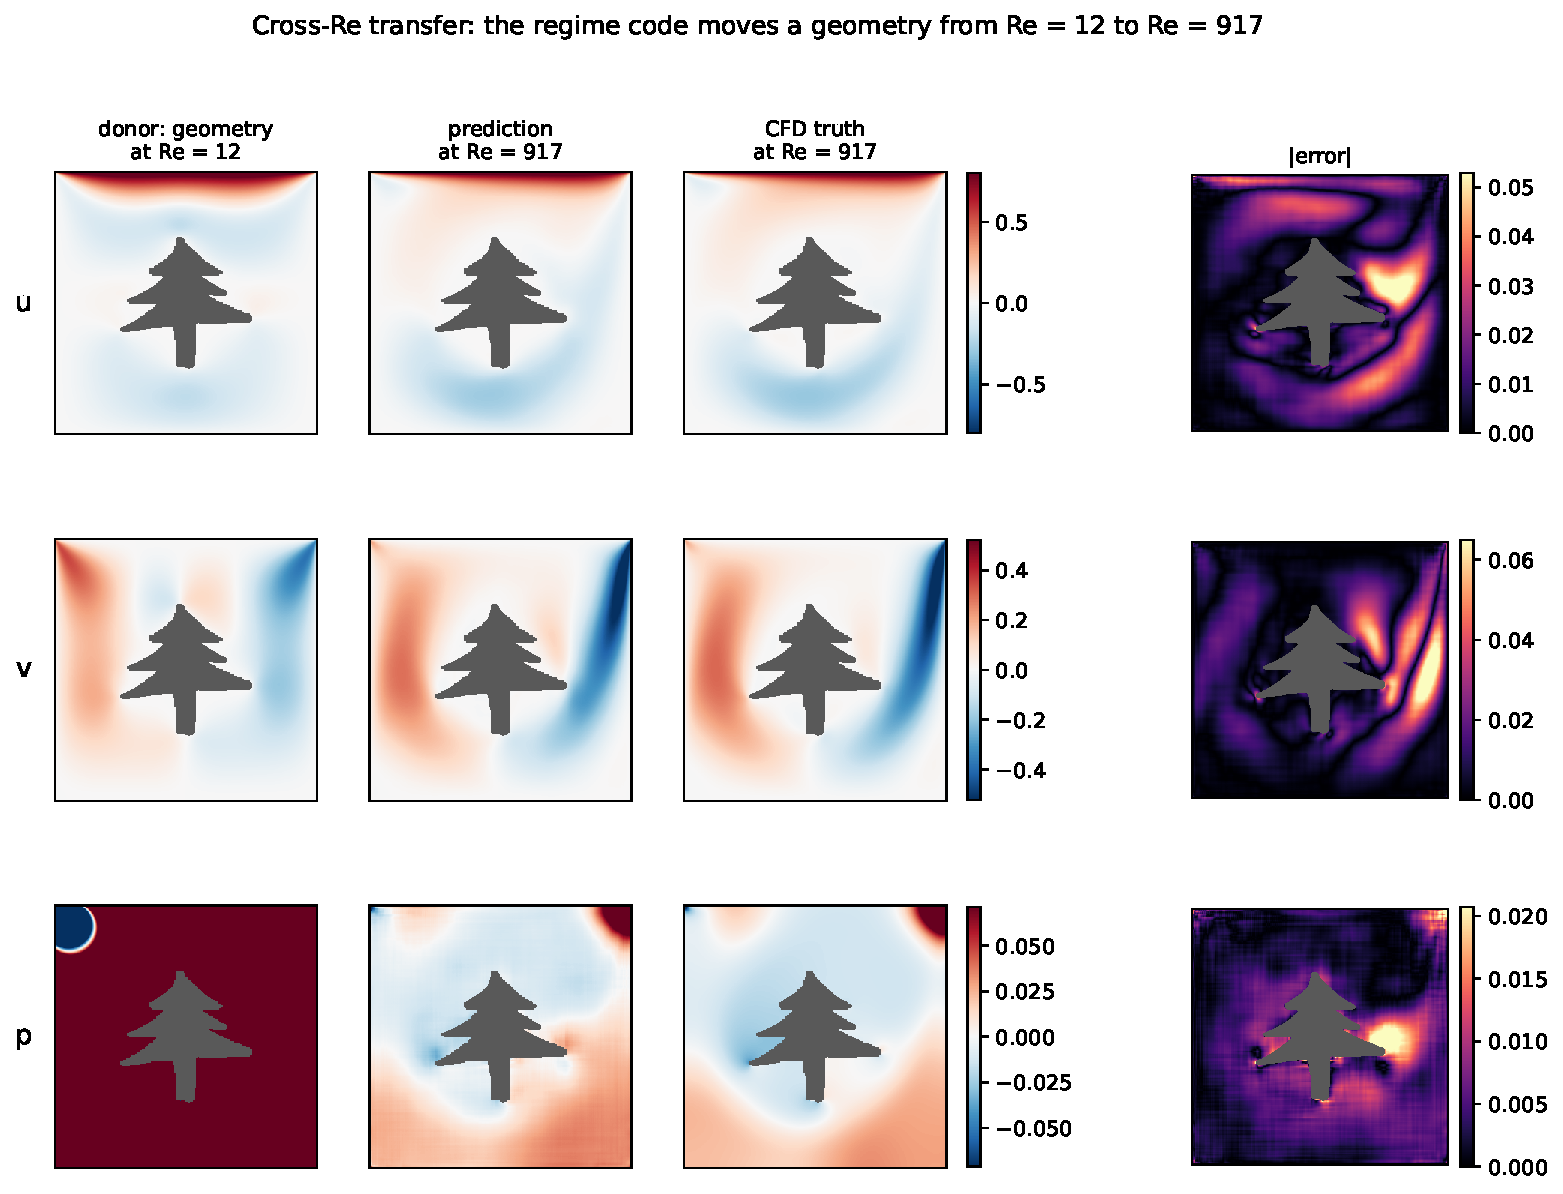
\includegraphics[width=\textwidth]{figures/transfer.pdf}
  \caption{Cross-Re transfer, visualized (Run 7 model). The model has
  encoded this geometry only at $\mathrm{Re} = 12$ (left column: the
  slow, diffuse, viscous-regime flow). Swapping in a regime code taken
  from a different sample at $\mathrm{Re} = 917$ and decoding produces
  the second column --- which develops the thin lid shear layer and the
  strong downwelling jet along the right wall, matching the CFD truth at
  $\mathrm{Re} = 917$ (third column) to within errors an order of
  magnitude smaller than the fields (fourth column). Color scales are
  set by the target fields, so the donor's pressure panel saturates:
  at $\mathrm{Re} = 12$ the nondimensional pressure is roughly fifty
  times larger, and the model correctly predicts this amplitude collapse
  across the Re jump. The regime code alone moved this geometry across
  two decades of Reynolds number.}
  \label{fig:transfer}
\end{figure}

\paragraph{The one prediction that failed --- instructively.} The
residual's Re content did not shrink; it \emph{grew}, from $0.243$ to
$0.692$. This is a squeezed balloon: in Run 6 the flow-encoded
$\boldsymbol{z}_{g}$ (32 dimensions) shared the burden of describing
Re-dependent flow appearance; now the field encoder has only
$\boldsymbol{z}_{\mu} + \boldsymbol{z}_{\xi}$ to describe the entire
flow, so the residual necessarily correlates with Re. The crucial
observation is that this does not matter functionally: transfer got
\emph{better} even though $\boldsymbol{z}_{\xi}$ is more Re-readable
than ever, and in the cross-Re swap the decoder still follows
$\boldsymbol{z}_{\mu}$ (donor error $0.574$ versus target error
$2.2 \times 10^{-3}$). The cross-Re training taught the decoder to
\emph{ignore} the Re content in the residual. This is the third
appearance of the document's central theme: what a block statistically
\emph{contains} (probe readability) and what the decoder functionally
\emph{uses} are different properties --- and the functional one is what
matters for composition and transfer.

\paragraph{Multi-seed confirmation.} Because Run 7 is the final
architecture, its numbers deserve the same treatment the earlier runs
received: two more seeds were trained and every metric is reported as
mean $\pm$ standard deviation (Table~\ref{tab:multiseed-run7}, with the
Run-6 multi-seed values alongside for comparison). Every headline claim
survives. The leak closure is seed-proof --- $-0.14 \pm 0.01$, negative
in every seed, and with the smallest error bar in the table, exactly as
expected for a property enforced by \emph{architecture} rather than
learned from data. The geometry recovery ($0.91 \pm 0.05$ versus Run 6's
$0.73 \pm 0.02$) and the transfer improvement ($1.48 \pm 0.09$ versus
$2.0 \pm 0.1$) are both real: the distributions do not overlap. The
donor test is remarkably tight ($0.573 \pm 0.002$): in every seed the
decoder takes the operating point from $\boldsymbol{z}_{\mu}$. And the
squeezed balloon behaves exactly as the functional-inertness
interpretation predicts: the residual's Re content has the
\emph{largest} error bar in the table ($0.60 \pm 0.11$, ranging from
$0.44$ to $0.69$ across seeds), yet the transfer ratio barely moves. If
the decoder actually used that Re content, transfer quality would swing
with it; it does not.

\begin{table}[htbp]
  \centering
  \caption{Run 7 multi-seed results: mean $\pm$ standard deviation over
  three random seeds, with the Run-6 multi-seed values (from
  Table~\ref{tab:multiseed}) for comparison. $^{\dagger}$Average of the
  three geometry-descriptor probes.}
  \label{tab:multiseed-run7}
  \begin{tabular}{lcc}
    \toprule
    Metric & Run 6 ($+$cross-Re) & Run 7 (static geometry) \\
    \midrule
    $\log \mathrm{Re}$ from $\boldsymbol{z}_{\mu}$ (want high)
      & $0.984 \pm 0.002$ & $0.966 \pm 0.015$ \\
    $\log \mathrm{Re}$ from $\boldsymbol{z}_{g}$ (want low)
      & $0.376 \pm 0.074$ & $\mathbf{-0.139 \pm 0.014}$ \\
    $\log \mathrm{Re}$ from $\boldsymbol{z}_{\xi}$ (want low, but inert)
      & $0.200 \pm 0.041$ & $0.596 \pm 0.110$ \\
    Geometry from $\boldsymbol{z}_{g}$ (want high)$^{\dagger}$
      & $0.732 \pm 0.018$ & $\mathbf{0.912 \pm 0.049}$ \\
    Same-Re swap ratio (want $\approx 1$)
      & $1.50 \pm 0.05$ & $1.33 \pm 0.10$ \\
    Cross-Re swap ratio (want $\approx 1$)
      & $2.0 \pm 0.1$ & $\mathbf{1.48 \pm 0.09}$ \\
    Cross-Re donor MSE (high = decoder follows $\boldsymbol{z}_{\mu}$)
      & $\approx 0.58$ & $0.573 \pm 0.002$ \\
    \bottomrule
  \end{tabular}
\end{table}

\subsection{Comparison against the published FlowBench baselines}

How good is the final model in absolute terms? The FlowBench benchmark
paper (Rabeh et al., \emph{Communications Engineering} 4:182, 2025)
evaluated eleven SciML models on exactly our dataset and split (2{,}400
train / 600 test, SDF representation, random split), reporting two
scores at $512^2$ resolution: \emph{M1}, the per-pixel MSE over the
fluid region converted to a $0$--$100$ scale via
$\mathrm{score} = -(100/6)\log_{10}(\mathrm{MSE})$, and \emph{M2}, the
same restricted to the boundary layer ($0 \le \mathrm{SDF} \le 0.2$).
We computed the identical metrics for the Run-7 model, upsampling its
$256^2$ output to $512^2$ before scoring (so the resolution difference
penalizes us, not the baselines). One fairness caveat is essential: the
baselines are \emph{operators} --- they predict fields from
$(\mathrm{SDF}, \mathrm{Re})$ alone. We therefore report two modes.
\emph{Reconstruction} encodes the target field itself and is only an
upper bound. \emph{Donor prediction} is the fair comparison: the model
receives the target's SDF (through the static geometry encoder) and one
example flow at the same Re from a \emph{different} geometry (supplying
$\boldsymbol{z}_{\mu}$ and $\boldsymbol{z}_{\xi}$) --- it never sees the
target's field. This mode covers the 373 of 600 test samples that have a
same-Re partner. Table~\ref{tab:baselines} reports the comparison.

\begin{table}[htbp]
  \centering
  \caption{Comparison against the published FlowBench baselines (SDF
  representation, random split, full training set; baseline scores from
  Table 1 of the benchmark paper). Higher is better; a $+10$ score
  difference corresponds to a $4\times$ lower MSE. Baselines are
  operators mapping $(\mathrm{SDF}, \mathrm{Re})$ to fields; our
  donor-prediction mode uses the target SDF plus one same-Re example
  flow from a different geometry; our reconstruction mode sees the
  target field and is an upper bound.}
  \label{tab:baselines}
  \begin{tabular}{llcc}
    \toprule
    Model & Type & M1 & M2 \\
    \midrule
    poseidon-T          & vision transformer (pretrained) & 64.9 & 73.3 \\
    scOT-T              & vision transformer              & 64.6 & 71.4 \\
    geometric-DeepONet  & neural operator                 & 53.0 & 59.9 \\
    DeepONet            & neural operator                 & 45.9 & 53.0 \\
    CNO                 & neural operator                 & 44.8 & 54.5 \\
    FNO                 & neural operator                 & 44.3 & 59.2 \\
    WNO                 & neural operator                 & 24.1 & 41.3 \\
    \midrule
    \textbf{Ours, donor prediction} & compositional autoencoder & 46.2 & 46.5 \\
    \textbf{Ours, reconstruction}   & (upper bound)             & 53.5 & 53.4 \\
    \bottomrule
  \end{tabular}
\end{table}

\paragraph{Reading the table.} In the fair donor-prediction mode, the
compositional model ($5.6$M parameters, trained at $256^2$, scored at
$512^2$) edges out every classical neural operator on global accuracy
--- DeepONet ($45.9$), CNO ($44.8$), FNO ($44.3$), WNO ($24.1$) ---
while trailing the much larger vision-transformer models
($\approx 65$). This satisfies the project plan's first success
criterion (accuracy comparable to the FlowBench baselines), and it does
so while providing what none of the baselines offer: a latent space with
separated, editable, transferable factors. The relative weakness is the
boundary layer: every baseline scores \emph{higher} on M2 than M1
(near-wall velocities are small, so boundary MSE is naturally lower),
whereas our M2 is flat ($\approx$ M1). We initially suspected our
$256^2$ native resolution; the follow-up experiment below shows the
real cause is subtler and more interesting.

\paragraph{Run 8: what the boundary loss buys --- and what it costs.}
To test whether the flat M2 could be fixed by loss design, Run 8 added
the boundary-layer weighted reconstruction loss (L3 of the working
notes) to the otherwise unchanged Run-7 recipe: a second reconstruction
term restricted to the band $0 \le \mathrm{SDF} \le 0.2$ and normalized
by the \emph{band's} own pixel count. The normalization is the point:
the band is only a few percent of the fluid pixels, so under the plain
loss its errors are diluted away; giving it its own average makes the
thin near-wall region worth as much as the entire rest of the fluid.
The result is a clean trade-off, visible from both ends. On the
reconstruction side L3 does exactly its job: M2 rises from $53.4$ to
$56.1$ and now sits \emph{above} M1 ($53.8$), reproducing the
$\mathrm{M2} > \mathrm{M1}$ pattern of the published baselines --- so
the flat M2 was \emph{not} a resolution ceiling but loss dilution. But
the compositional properties pay for it: donor prediction drops from
$46.2$ to $39.7$, the cross-Re transfer ratio degrades from
$1.48 \pm 0.09$ to $2.86$, and the residual's Re content rises to
$0.77$ --- and this time the readability is \emph{not} inert. The
mechanism is coherent: to nail near-wall detail the decoder learns to
lean on the sample-specific content of $\boldsymbol{z}_{\xi}$, and
donor prediction and swaps are exactly the modes where
$\boldsymbol{z}_{\xi}$ comes from a different sample. Boundary-layer
fidelity and compositional recombinability compete for the same decoder
capacity, and L3 buys one with the other. Since transfer is this
study's central property, Run 7 remains the final model, and we accept
its flat M2 as the price of a latent space that recombines.

\section{Status and next steps}

\paragraph{Implemented and validated.} The block-structured autoencoder
with regime and geometry supervision (Runs 1--3); group-structured
minibatches and the same-factor invariance loss L10 (Run 4); the
swap-consistency loss L12 (Run 5); and a diagnostic suite comprising
linear probes, same-Re swap error, and cross-Re swap error --- all
runnable on stored checkpoints without retraining. Also complete: the
cross-Re swap promoted from diagnostic to training loss (Run 6), which
took the transfer test from a two-orders-of-magnitude failure to near
reconstruction quality. The multi-seed protocol (three seeds per
configuration, Table~\ref{tab:multiseed}) is also complete and confirms
the headline findings with error bars: \emph{statistical decorrelation
cannot functionally separate the blocks at any weight; the structural
losses achieve separation (L10), recombinability (L12, $1.04 \pm 0.03$),
and transfer (cross-Re swap, $2.0 \pm 0.1$ versus $\sim\!170$ without
it) at essentially no cost to reconstruction}. The three properties are
genuinely distinct: each required its own loss, and each is invisible to
the other properties' diagnostics.

Concept-vector arithmetic (Table~\ref{tab:concept}) is also complete:
the geometry directions act as clean edit handles (cross-talk
$\le 0.11$), and the block-restricted variant traced the remaining
Re-to-geometry cross-talk to the encoder inferring object position from
Re-dependent flow structures. That hypothesis was then confirmed
decisively by Run 7 (Table~\ref{tab:probes-run7}): with a static
geometry encoder reading the SDF, the $\boldsymbol{z}_{g}$ leak closes
exactly, geometry recovery jumps to $0.93$--$0.98$, transfer improves to
$1.42$, and the concept-vector cross-talk vanishes. Run 7 is the final
architecture for this study, and its numbers now carry error bars: the
three-seed protocol (Table~\ref{tab:multiseed-run7}) confirms the leak
closure ($-0.14 \pm 0.01$), the geometry gain ($0.91 \pm 0.05$), and the
transfer improvement ($1.48 \pm 0.09$) as seed-robust effects.

Finally, the field visualizations are in place: a reconstruction example
from the final model (Figure~\ref{fig:recon}) and the cross-Re transfer
showcase (Figure~\ref{fig:transfer}), which shows the regime code moving
a geometry across two decades of Reynolds number --- including the
correct collapse of the pressure amplitude --- with errors an order of
magnitude below the fields. The comparison against the published
FlowBench baselines (Table~\ref{tab:baselines}) is also complete: in the
operator-comparable donor-prediction mode the model edges out every
classical neural operator on global accuracy (M1 $= 46.2$ vs.\
$44$--$46$), satisfying the project plan's first success criterion.
The boundary-layer weakness (flat M2) was then diagnosed by Run 8: the
L3 boundary-weighted loss fixes it in reconstruction (M2 $53.4 \to
56.1$) but degrades transfer ($1.48 \to 2.86$) --- boundary fidelity
and recombinability compete for decoder capacity, so Run 7 remains the
final model.

\paragraph{Planned increments, in order.}
%
\begin{itemize}
  \item \textbf{Physics/spectral loss family}: PDE residual (L18) and/or
        spectrum matching (L22), the one loss family not yet ablated.
  \item \textbf{Residual capacity}: shrink the residual block (e.g.\
        $16 \to 4$ dimensions). In Run 7 the residual is Re-readable
        ($R^2 \approx 0.6$) but functionally inert; a smaller block
        would test whether the readability is even necessary.
  \item \textbf{Loss library extensions}: HSIC (L7), which detects
        nonlinear dependence between blocks, not just linear correlation.
  \item \textbf{Architecture}: an INR-style implicit decoder, which can
        be queried at any spatial point rather than on a fixed grid.
  \item \textbf{Beyond steady flow}: the dynamics block
        $\boldsymbol{z}_{\eta}$ and a latent time-stepper $\Phi$ for
        time-dependent cases (the framework's Path B/C), moving toward
        the warm-up and Case-1 studies of the anchor paper.
\end{itemize}

\newpage

\appendix

\section{Appendix: Running the code on Nova cluster}

\begin{enumerate}
  \item Log in to the Nova cluster:
        \texttt{ssh username@nova.its.iastate.edu}
  \item Activate the virtual environment that contains the required
        packages.
  \item Request a resource allocation:
        \texttt{salloc -N 1 -n 4 -t 01:00:00 --gres=gpu:a100 --mem 369G}
  \item Train:
        \texttt{python main.py --config configs/compositional/conf.yaml}
  \item Run the diagnostics on a checkpoint (linear probes and swap
        errors; \texttt{version\_N} is printed at the end of training):
        \begin{verbatim}
python diagnostics/probes.py \
  --config configs/compositional/conf.yaml \
  --checkpoint checkpoints/compositional/version_N/last.ckpt
        \end{verbatim}
\end{enumerate}

\end{document}
